\documentclass[12pt]{article}
\usepackage[letterpaper,margin=1in,footskip=.5in]{geometry}
\usepackage{setspace}
\onehalfspacing
\usepackage{graphicx,amsmath,amssymb,booktabs,threeparttable,float,tabularx,longtable,ragged2e}
\usepackage[round,sort]{natbib}
\usepackage[T1]{fontenc}
\usepackage[utf8]{inputenc}
\usepackage{lmodern,microtype,textcomp,caption}
\captionsetup{font=small,labelfont=bf,justification=justified,singlelinecheck=false}
\usepackage[colorlinks=true,linkcolor=blue,citecolor=blue,urlcolor=blue]{hyperref}
\newenvironment{tablenoteblock}{\begin{tablenotes}[flushleft]\footnotesize\item[]\justifying\textnormal{Note:}\ }{\end{tablenotes}}
\setlength{\parindent}{2em}
\setlength{\emergencystretch}{2em}
\title{Communication matters: investor-manager interactions and asset pricing}
\author{Chenzhao Jia\\[.3em]\small Supervision team: Tianlun Fei, Ying Jiang, Xiaoquan Liu}
\date{October 23, 2026\\\small Integrated working draft}
\begin{document}
\maketitle
\begin{abstract}
We examine whether public investor inquiries and managerial replies contain information about stock returns in China. The Effective Sentiment Index (ESI) combines investor tone scaled by attention with managerial tone weighted by reply substantiveness and the preceding investor sentiment state. Recomputing the historical question-date specification, equal- and value-weighted long-minus-short portfolios earn gross daily open-to-close excess returns of 5.31 and 5.26 basis points, respectively, exceeding the corresponding point estimates for either tone alone. The one-day ESI coefficient remains positive after controls and firm and date effects. These results are retrospective: subsequent replies are assigned to question dates, and the original implementation uses full-period scales and future trading-status information. In separate public-availability tests, ESI remains positively associated with returns on its own, but the complete text horse race and value-weighted risk-adjusted performance are not significant. Actual announcement-date earnings tests do not establish a fundamental-information channel. Full-corpus content classification provides descriptive and exploratory evidence, with no significant joint differences in ESI slopes across topics. The findings support a positive historical association while limiting claims about independent information, mechanisms, and implementable trading gains.
\end{abstract}
\noindent\textbf{Keywords:} investor sentiment; managerial tone; investor relations; textual analysis; asset pricing.
\clearpage
\section{Introduction}\label{sec:introduction}
Investor opinions and managerial disclosures can both contain information relevant to stock prices. Studies of investor text examine expressed beliefs on financial social media \citep{chen2014,bartov2018,cookson2024}, while studies of corporate language examine the information and beliefs conveyed by managers \citep{li2010,jiang2019}. Considering either side alone leaves a question unanswered: does the combination of an investor's concern and the corresponding managerial reply convey return information beyond the two tones separately? A positive reply to an anxious, specific question need not have the same meaning as equally positive language in a generic exchange.

Interactive platforms make this question observable. Investors choose what to ask, and managers decide whether and how to respond. Inquiries can elicit additional details, while the specificity of replies can help readers interpret management's language \citep{hollander2010,matsumoto2011}. At the same time, questions and replies can react to previous prices or reflect strategic disclosure. We therefore distinguish the predictive association of a dialogue measure from evidence that replies cause price changes or disclose previously unknown fundamentals.

The Chinese market provides a setting in which to compare information in public dialogue with possible trading pressure. The Shenzhen and Shanghai exchanges operate interaction platforms covering a broad cross section of listed firms \citep{lee2022shall}. Substantial retail participation connects these communications to investor trading, and short-sale constraints may limit the offsetting response of arbitrageurs \citep{liao2022,jiang2022}. Neither observation by itself establishes irrational sentiment. Chinese prices can also contain information about future fundamentals \citep{carpenter2021}. The distinction between information and pressure is consequently an empirical question rather than an assumption about the market.

We construct the Effective Sentiment Index (ESI) from matched investor inquiries and managerial replies. Investor tone supplies the signed investor component, scaled by question volume. The managerial component combines standardized reply tone with reply substantiveness and a smooth weight determined by the preceding investor tone. The same managerial tone can therefore receive different weights depending on what investors asked and how specifically managers responded. The weights are maintained modeling choices; their economic motivation does not establish that they are optimal.

The historical question-date analysis reproduces the Annual Review program using its frozen rules. Equal-weighted (EW) and value-weighted (VW) ESI portfolios earn gross daily O2C excess returns of 5.31 and 5.26 basis points, respectively. Under the original arithmetic annualization convention these are 12.85\% and 12.72\%. Both exceed the corresponding point estimates for investor tone or manager tone alone. ESI also has a positive one-day regression coefficient after the original controls and fixed effects. These comparisons describe historical associations: the original pools and factor alignment are retained, and replies recorded after the question date enter that date's signal.

We separately examine the information clock using existing public-availability C2C results. In a common sample, the standalone ESI coefficient is 1.48 basis points ($t=4.36$), but falls to 0.58 ($t=0.75$) after including the complete set of text features. On common portfolio dates and a common candidate pool, the EW China four-factor alpha is 4.68 basis points ($t=3.29$), while the VW alpha is 3.78 ($t=1.54$). These results do not support a stable advantage over manager tone. The C2C extension uses a different frozen calibration and later sample, so the change cannot be attributed solely to reply timing.

Two additional analyses qualify the interpretation. Signals observed before actual earnings announcements do not significantly predict standardized unexpected earnings or announcement returns in the available tests. Full-corpus automated classification describes 19 content themes and five question natures, but joint tests do not reject equal ESI slopes across topics. A significant products-or-business slope in the baseline topic regression loses significance after both tones enter. We retain these results because they distinguish the positive historical association from the stronger claims needed to identify a mechanism.

The study contributes in three ways. First, it develops a dialogue-based sentiment measure that makes attention, reply specificity and the investor state explicit. This differs from treating a reply as standalone managerial language or simply summing two tone scores. Second, it compares the measure with its component signals and separates retrospective O2C evidence from public-availability regressions and common-pool portfolios. This clarifies which conclusions depend on the information clock and competing text information. Third, it brings content and question-nature classifications into the interpretation of interactive disclosures. These classifications describe what investors ask and what managers discuss; they are not taken as independently validated semantic labels or evidence of different priced risks.

Section~\ref{sec:literature_review} reviews related work. Section~\ref{sec:data} describes the data and ESI. Section~\ref{sec:baseline_return_predictability} reports historical return evidence. Section~\ref{sec:supplements} presents the public-availability, earnings and topic evidence, and Section~\ref{sec:conclusion} concludes.

\section{Literature review}\label{sec:literature_review}

\subsection{Investor sentiment}


Empirical asset pricing studies debate whether investor sentiment introduces transient noise or predicts fundamentals. \citet{delong1990noise} develop a theoretical model to demonstrate that unpredictable changes in noise trader beliefs could move prices away from fundamental values. To study how investor sentiment affects the cross section of stock returns, \citet{baker2006} construct a composite index from market proxies \footnote{The index includes discounts on closed end funds, NYSE turnover, the number of IPOs, returns on the first trading day, the equity share in new issues, and the dividend premium.} and show that high sentiment predicts lower returns, specifically for stocks that are difficult to value and arbitrage. Subsequent research extends these indirect measures to international markets \citep{baker2012global,schmeling2009} \footnote{\citet{baker2012global} construct composite sentiment indices for six international markets and show that global and local sentiment components predict future stock returns. \citet{schmeling2009} uses consumer confidence across 18 countries to measure investor sentiment and predict future returns.} and other asset classes including government bonds, commodities, and index options \citep{baker2012bonds,gao2015,han2008}.\footnote{\citet{baker2012bonds} find that stock market sentiment predicts the excess returns of government bonds. \citet{gao2015} construct a composite index from market proxies using the partial least squares method to explain the returns and comovements of commodity futures. \citet{han2008} show that market pessimism steepens the volatility smile and increases negative skewness for index options.} These indirect measures often capture unrelated market noise, making their predictive power dependent on the choice and aggregation of proxies \citep{huang2015}.

Textual analysis measures sentiment from expressed opinions rather than market outcomes, although model and sample choices still affect the measurement. Early textual analysis research on investor sentiment aligns with the transient noise perspective. \citet{tetlock2007giving} analyzes a daily market column from the Wall Street Journal and shows that media pessimism predicts price declines followed by reversals, which indicates temporary price pressure instead of fundamental information.


By measuring investor sentiment from text on social media, subsequent studies challenge the transient noise view. \citet{chen2014} analyze Seeking Alpha articles and comments to show that these opinions predict future stock returns and earnings surprises. This evidence suggests that social media platforms can aggregate dispersed information about firm value rather than merely generating random chatter. \citet{bartov2018} find similar results using Twitter data, showing that individual tweets posted before earnings announcements predict forthcoming earnings and returns. Recent research evaluates the economic magnitude of textual signals through portfolio construction. \citet{ke2021predicting} and \citet{lopez2023chatgpt} extract sentiment from financial news to form portfolios and document return predictability. \citet{ke2021predicting} show that the incorporation delay is longer for small stocks. \citet{lopez2023chatgpt} interpret subsequent drift through information processing constraints and limits to arbitrage.

One possible source of these conflicting findings is that sentiment and attention capture distinct dimensions of investor behavior. Traditional market proxies often conflate these two dimensions as they are based on the same aggregate trading outcomes. For example, \citet{baker2006} use market turnover to construct a sentiment index, whereas \citet{barber2008} and \citet{da2011} interpret abnormal trading volume and extreme returns as indirect proxies for investor attention. This overlap implies that trading metrics cannot distinguish the direction of investor sentiment from the intensity of attention or other liquidity factors. Textual data separate these dimensions by using linguistic tone to measure opinions and message volume to measure attention \citep{antweiler2004}. \citet{cookson2024} address this issue by analyzing messages from StockTwits, Twitter, and Seeking Alpha. By separating textual sentiment from message volume, they demonstrate that sentiment contains information relevant to stock prices, whereas attention reflects retail buying pressure and price overreaction.

\subsection{Managerial sentiment}

Managers possess private information about firm prospects, and investors use managerial disclosures to assess firm fundamentals \citep{beyer2010financial,healy2001information}. However, managerial tone can reflect both information and managers' subjective beliefs about firm prospects. On the one hand, tone reflects cognitive biases. Using an aggregate manager sentiment index, \citet{jiang2019} show that optimism predicts lower future aggregate returns and earnings surprises. They also document links between manager sentiment, extrapolation of recent performance, and overinvestment. \citet{chen2018morning} observe that the tone of earnings conference calls becomes more negative later in the day and that investors temporarily overreact to this variation. On the other hand, managerial tone can convey information about future economic conditions. At the macroeconomic level, \citet{demers2024aggregate} demonstrate that positive changes in earnings announcement tone predict economic growth in the following quarter. This evidence suggests that corporate tone also contains information relevant to firm value and future stock returns.

Specific details help investors evaluate whether fundamental information supports managerial tone.  \citet{crawford1982} develop a model to show that conflicts of interest between a sender and a receiver make vague communication unreliable. Since managers have incentives to exaggerate firm prospects, their optimism lacks credibility. In this case, investors tend to place more weight on managerial tone when specific and verifiable information supports the response. Using management earnings forecasts, \citet{hutton2003} report that positive forecasts provide information only when managers include verifiable statements about future performance. \citet{baginski2016verification} analyze management press releases and reveal that quantitative forecast news strengthens the market response to linguistic tone, whereas imprecision weakens the response. 

Managerial communication may also affect how investors perceive firm risk. \citet{gennaioli2015} develop a model of delegated asset management in which trust in fund managers reduces perceived risk and increases investor willingness to hold risky assets. \citet{germann2025trust} test this mechanism in an experimental setting and conclude that greater trust in a fund manager increases confidence and allocations to risky assets. These findings motivate testing whether the return association of managerial replies varies with the sentiment expressed in the preceding inquiry. \citet{loewenstein2001risk} argue that emotional states affect risk judgments. Specifically, anxiety shifts attention toward threats and increases an individual's tendency to seek and rely on external advice \citep{eysenck2007anxiety,gino2012}. These findings suggest that investors evaluate the same managerial reply differently depending on their initial sentiment state.

\subsection{Investor-manager interaction}

Interactive settings may provide corporate information beyond standard disclosures. First, interactive environments reveal additional fundamental details as they allow investors to publicly request specific information \citep{hollander2010}. In traditional disclosures, managers determine the content based on their internal expectations of investor demand. \citet{matsumoto2011} examine over 10,000 earnings calls from 2003 to 2005 to separate prepared presentations from discussion sessions. Using intraday absolute returns, they demonstrate that discussions contain more information than prepared presentations as external questions prompt managers to reveal new details.

Second, the way managers respond to explicit questions provides an additional pricing signal to the market. Response behavior affects prices through direct market reactions and subsequent information production. Investors may directly interpret a refusal to answer as a lack of transparency. \citet{hollander2010} examine individual requests during earnings calls and document that managerial refusal to answer questions is associated with negative intraday stock reactions. Rather than directly refusing to answer, managers often use evasive language to withhold sensitive information \citep{gow2021}. \citet{lee2016} evaluates how managers rely on scripted responses during discussions, reporting that this behavior predicts negative stock returns and lower future operating performance. Similarly, \citet{xie2023} show that boilerplate replies on Chinese platforms occur more frequently during weak firm performance and correlate with reduced market liquidity. Evasive responses can also restrict information production by external intermediaries. \citet{boustanifar2025} report that evasive replies precede less original reporting from professional media. With less substantive content to analyze, reduced media coverage restricts investor engagement and is associated with weaker abnormal returns.


Recent studies examine interactive platforms to understand their market implications. \citet{lee2022shall} analyze approximately 2.5 million investor questions and corporate replies on Chinese IIPs from 2010 to 2017. Using manual annotations and language algorithms, they evaluate the nature of investor questions and measure the level of interaction through platform activity. They find that most questions reflect the difficulties investors face when integrating existing public information. Their results show that greater platform activity is associated with higher market liquidity, narrower trading spreads, and greater price informativeness, suggesting that interactions lower information processing costs. Related research extends these platform activity metrics to corporate outcomes, showing a positive relationship with corporate investment efficiency \citep{xu2024}. 

We construct the Effective Sentiment Index (ESI) from matched investor inquiries and managerial replies on IIPs. The index accounts for the investor's preceding sentiment and whether the managerial response provides substantive information. We then test whether this interaction measure predicts stock returns beyond investor tone and managerial tone considered separately.




\section{Data and descriptive characteristics}\label{sec:data}
\subsection{Sources, sample and the information clock}
Our textual inputs are public Q\&A records from the Shenzhen Stock Exchange's Easy Interaction platform and the Shanghai Stock Exchange's E-Interaction platform, obtained through CNRDS. The source supplies matched questions and replies. Stock returns, prices, financial characteristics, trading variables and listing dates come from CSMAR. We preserve the source records, production tone scores and Random Forest substantiveness scores; the integration does not retrain the classifiers or alter historical observations.

The original regression preparation retains 5,812,275 firm-day observations after its listing-age filter. ESI has complete text inputs on 1,317,473 of these observations. The original portfolio preparation has 2,553,356 complete-text observations and follows a different eligibility rule. These counts describe input pools, not final regression samples or independent questions. Table~\ref{tab:parameters} reports their separate scales. A firm day with at least one recorded inquiry is an interaction day; absence of a question is not a neutral tone. Missing tone or reply inputs are not filled with zero to manufacture an ESI observation.

Reply timing matters because an answer may arrive after the investor's question. In the historical construction, both sides of the matched dialogue are aggregated to the original company-question-date cohort. This is not separate aggregation of all questions posted today and all replies posted today. A Day~1 question and its Day~3 reply contribute to the historical Day~1 ESI, even though the completed signal was not available on Day~1. Returns attached to that question date need not follow the public release of all inputs.

The separate availability construction assigns a completed cohort to the first exchange trading day strictly after its last recorded reply; multiple cohorts arriving at the same company-availability date are combined. We denote this date by $a$ when defining its outcomes. This extension changes the clock and uses its own frozen calibration and sample. Neither construction treats an unanswered question as a completed matched dialogue.

\subsection{Construction and interpretation of ESI}\label{sec:esi_construction}
ESI combines two signed components: attention-weighted investor tone and content-weighted managerial tone. Figure~\ref{fig:esi_flow} gives the sequence before the individual steps. The aim is to represent the interaction context explicitly, not to claim that the index measures a directly observed psychological response.
\begin{figure}[H]\centering\small
\fbox{\parbox{.91\textwidth}{\centering Matched question and reply records\\Retain the original question-date cohort; distinguish later public availability}}
\par\smallskip$\Downarrow$\par\smallskip
\fbox{\parbox{.91\textwidth}{\centering Score and aggregate both tones; measure question volume and reply substantiveness}}
\par\smallskip$\Downarrow$\par\smallskip
\fbox{\parbox{.91\textwidth}{\centering Investor component: $I(1+\lambda A)$\\Managerial component: $Z^M Sub K(I)$, with original asymmetric protection}}
\par\smallskip$\Downarrow$\par\smallskip
\fbox{\parbox{.91\textwidth}{\centering Combine using frozen full-pool text scales\\Evaluate historical O2C outcomes; report availability C2C evidence separately}}
\caption{From Matched Dialogue to the Historical ESI}\label{fig:esi_flow}
\end{figure}
Separate sentiment classifiers produce negative, neutral and positive probabilities for inquiries and replies. Tone is the positive probability minus the negative probability, ranging from $-1$ to $1$. We average the respective scores within the matched firm-date cohort. Contextual scoring recognizes that financial expressions can differ from general language \citep{loughran2011}; this motivation does not establish the accuracy of the undocumented production sentiment models.

Reply substantiveness, $Sub_{i,t}$, is one minus the Random Forest probability of an evasive reply. Its inputs include lengths, Q\&A similarity, numerical and date indicators, and generic-disclosure phrases. The existing label file provides 1,999 usable substantiveness labels but lacks sufficient annotation metadata to establish independent ground truth. Appendix~\ref{app:nlp_methodology} reports a common-holdout comparison with Chinese BERT and a local instruction model. The production scores remain unchanged.

Let $I_{i,t}$ and $M_{i,t}$ denote the two mean tones, and $N_{i,t}$ the number of questions. Define
\begin{align}
A_{i,t}&=\frac{\log(1+N_{i,t})}{\max_{j,s}\log(1+N_{j,s})}, & Z^M_{i,t}&=\frac{M_{i,t}-\bar M}{\sigma_M},\\
\theta&=Q_I(0.30), & \sigma_K&=0.8\sigma_I,\\
K(I_{i,t})&=\exp\!\left[-\frac{(I_{i,t}-\theta)^2}{2\sigma_K^2}\right], & G_{i,t}&=Z^M_{i,t}Sub_{i,t}K(I_{i,t}).
\end{align}
The attention multiplier preserves investor tone's sign and lies between 1 and 1.5 when $\lambda=0.5$. Attention and tone describe distinct aspects of expressed beliefs \citep{barber2008,da2011,cookson2024}. Reply specificity moderates the contribution of managerial language, consistent with examining verifiable detail rather than optimism alone \citep{hutton2003,hollander2010}. The state weight is largest at the 30th percentile of investor tone and falls with distance. This is a modeling choice motivated by the possibility that initial affect changes how advice is processed \citep{gino2012,loewenstein2001risk}; those studies do not identify our numerical anchor or bandwidth.

The original code contains an asymmetric protection, which must also appear in the written formula:
\begin{equation}
\widetilde G_{i,t}=\begin{cases}0,& I_{i,t}>0\ \text{and}\ G_{i,t}<0,\\G_{i,t},&\text{otherwise},\end{cases}
\quad ESI_{i,t}=I_{i,t}(1+0.5A_{i,t})+5\widetilde G_{i,t}.\label{eq:esi}
\end{equation}
Below-average managerial tone therefore does not subtract from a positive investor component in that state. This truncation is a historical specification choice, not an estimated behavioral result.

Table~\ref{tab:parameters} uses the full original 2010--2024 text pools before response-lag grouping. Regression and portfolio programs use different pools; their separate means, standard deviations, anchors and attention denominators are preserved. The constants $\lambda=0.5$, $\gamma=5$, $q=0.30$ and $b=0.8$ are inherited choices. Full-sample moments explain how they translate into weights; they do not demonstrate optimality, preregistration, or an untouched out-of-sample test. Figures~\ref{fig:parameter_distribution} and \ref{fig:weights} show the distributional scale and weighting function.
\begin{table}[H]
\centering\footnotesize
\caption{Frozen Full-Sample Text Scales}\label{tab:parameters}
\begin{threeparttable}
\renewcommand{\arraystretch}{1.12}
\begin{tabular*}{\textwidth}{@{\extracolsep{\fill}}lrr@{}}
\toprule
Quantity & Regression pool & Portfolio pool \\
\midrule
Complete text observations & 1,317,473 & 2,553,356 \\
$\bar M$ & 0.1868 & 0.1690 \\
$\sigma_M$ & 0.2796 & 0.2693 \\
$Q_I(0.30)$ & -0.1417 & -0.2169 \\
$\sigma_I$ & 0.3659 & 0.3761 \\
$0.8\sigma_I$ & 0.2928 & 0.3009 \\
$\max\log(1+N)$ & 4.8040 & 5.5134 \\
$\overline{ESI}$ & 0.4857 & 0.3609 \\
$\sigma_{ESI}$ & 2.8106 & 2.5182 \\
\bottomrule
\end{tabular*}
\begin{tablenoteblock}
The original 2010--2024 analysis pools are retained separately. Regression construction excludes the first six months after listing; portfolio preparation uses its original return and market-capitalization availability rules. These are full-sample distributional scales, not an early training window or externally estimated economic parameters. $\lambda=0.5$, $\gamma=5$, $q=0.30$, and $b=0.8$ remain fixed. No per-lag recalibration is performed. The full-period construction overlaps the evaluation period.
\end{tablenoteblock}
\end{threeparttable}
\end{table}

\begin{figure}[H]\centering
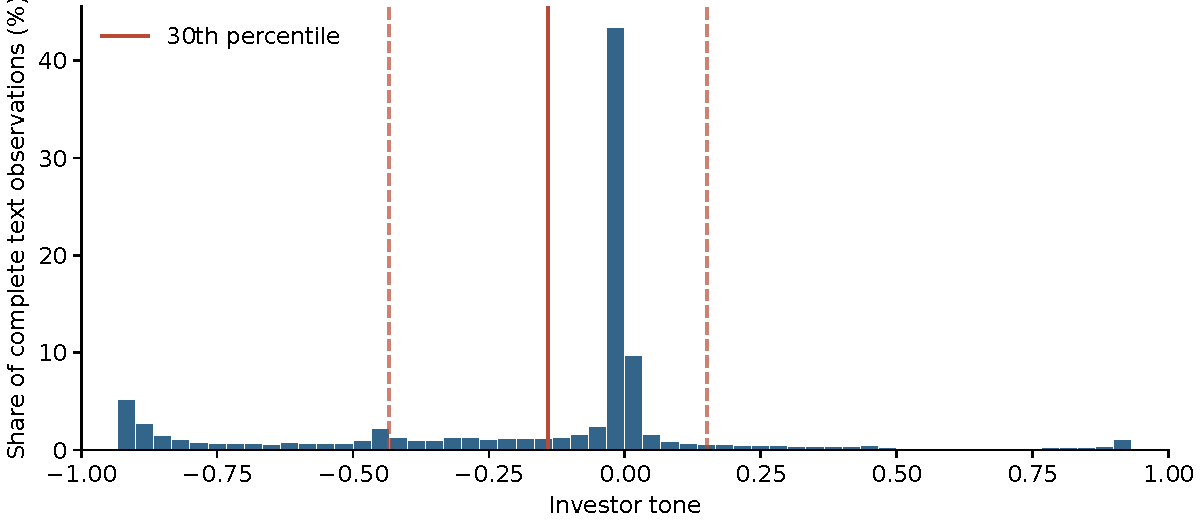
\includegraphics[width=\textwidth]{figures/investor_distribution.pdf}
\caption{Full-Regression-Pool Investor Tone and the State Anchor}\label{fig:parameter_distribution}
\footnotesize Complete text observations in the original regression pool. The solid line is the frozen 30th percentile; dashed lines are one kernel bandwidth on either side. Frequencies are descriptive and do not use returns.
\end{figure}
\begin{figure}[H]\centering
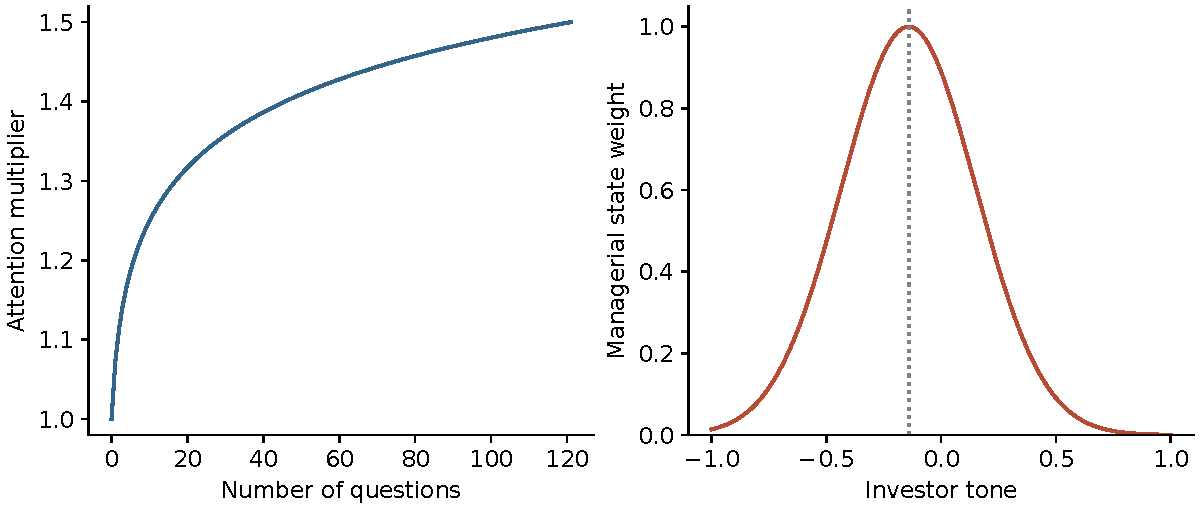
\includegraphics[width=\textwidth]{figures/esi_weights.pdf}
\caption{Historical Attention Multiplier and State Weight}\label{fig:weights}
\footnotesize Curves apply frozen regression-pool scales. The state curve is a deterministic weight, not a density estimate or fitted return response. Both pool-specific scale sets appear in Table~\ref{tab:parameters}.
\end{figure}

\subsection{Outcome and control definitions}
The historical O2C outcome is the next recorded stock day's closing price divided by its opening price minus one, less that record's risk-free rate. Excluding the overnight interval does not solve the late-reply problem. Original factor-residual outcomes use full-period firm regressions with factors indexed by the signal date. They are in-sample residuals, not rolling estimates based solely on past data.

Historical baseline regressions use eleven controls: size, book-to-market, profitability, leverage, illiquidity, turnover, prior return, trailing volatility, earlier cumulative returns, prior news tone and a news indicator. Table~\ref{tab:variables} groups them by use. News controls distinguish platform language from the prior public-information environment. Accounting inputs are inherited from the master panel; this integration does not reconstruct point-in-time revisions or publication histories. Announcement-specific controls are defined in their test rather than mixed into the baseline data description.

\section{Historical return evidence}\label{sec:baseline_return_predictability}
\subsection{Portfolio sorts}
We reproduce the Annual Review program with the original scores, sign restrictions, quantile cutoffs, position limits and eligibility rules. The long leg contains up to 50 positive-signal stocks in the upper 30 percent of the daily distribution; the short leg contains up to 50 negative-signal stocks in the lower 30 percent. Both legs must exist. EW portfolios give equal weight within each leg; VW portfolios use the original market-capitalization weights.

Table~\ref{tab:horse_race} reports gross ESI returns of 5.31 basis points per day with equal weights ($t=5.95$) and 5.26 with value weights ($t=3.57$). Arithmetic annualized returns are 12.85\% and 12.72\%. Investor-tone portfolios earn 4.43 and 4.38 basis points; manager-tone portfolios earn 2.48 and 2.75. ESI has the largest point estimate among these three signals under both weights. Separate significance levels and unequal candidate pools do not establish that differences are statistically significant.

The domestic CH4 model includes market, size, value and sentiment factors \citep{liu2019}. The historical q5 comparison uses the U.S. Global-q augmented q-factor series \citep{hou2021}; it is not a Chinese CSMAR factor set. ESI alphas are positive under both benchmarks. The original signal-date factors and daily intervals differ from next-record intraday returns, so these are diagnostic historical alphas. The availability comparison separately reports domestic CH4 and domestic FF3 over aligned holding dates.

The original program excludes stocks according to their next recorded closing-limit status, which is unavailable at signal-date portfolio formation. Together with full-period scales and retrospective reply assignment, this prevents interpretation as attainable trading profits. The short leg is theoretical, and returns exclude trading, borrowing and market-impact costs. Recomputed values replace old printed figures without changing parameters to make them coincide.
\begin{table}[H]
\centering\footnotesize
\caption{Historical O2C Portfolio Performance}\label{tab:horse_race}
\begin{threeparttable}
\renewcommand{\arraystretch}{1.12}
\begin{tabular*}{\textwidth}{@{\extracolsep{\fill}}lrrrrr@{}}
\toprule
Signal & Mean (bps) & Annual (\%) & Sharpe & CH4 $\alpha$ & U.S. q5 $\alpha$ \\
\midrule
ESI (EW) & 5.31 (5.95) & 12.85 & 1.54 & 5.17 (5.74) & 5.42 (6.06) \\
Investor tone (EW) & 4.43 (4.22) & 10.73 & 1.11 & 4.73 (4.55) & 4.60 (4.34) \\
Manager tone (EW) & 2.48 (2.83) & 6.00 & 0.71 & 2.36 (2.65) & 2.46 (2.80) \\
ESI (VW) & 5.26 (3.57) & 12.72 & 0.91 & 5.16 (3.46) & 5.40 (3.67) \\
Investor tone (VW) & 4.38 (2.70) & 10.59 & 0.69 & 4.73 (2.88) & 4.51 (2.79) \\
Manager tone (VW) & 2.75 (1.79) & 6.66 & 0.45 & 2.73 (1.77) & 2.69 (1.75) \\
\bottomrule
\end{tabular*}
\begin{tablenoteblock}
Gross long-minus-short returns; 3,642 dates for each row. Parentheses contain HAC(5) $t$ statistics. Up to 50 positive-signal stocks in the upper 30 percent form the long leg; up to 50 negative-signal stocks in the lower 30 percent form the short leg. Both legs must exist. Annualization is the historical arithmetic convention, $242\bar r\times100$, with Sharpe scaled by $\sqrt{242}$. Candidate pools are signal-specific, not a common-stock-pool horse race. Next-record O2C excess returns, future closing-limit exclusions, full-period text scales, and signal-date factors reproduce the original implementation. CH4 is domestic; q5 is the U.S. Global-q series. The intraday outcome and daily factor intervals differ. These are historical diagnostic alphas, not implementable profits. All figures are recomputed values rather than copied PDF numbers.
\end{tablenoteblock}
\end{threeparttable}
\end{table}


\subsection{Return regressions}
The historical baseline estimates
\begin{equation}
y^{O2C}_{i,t+1}=\alpha_i+\delta_t+\beta Z^{ESI}_{i,t}+\boldsymbol c_{i,t}'\boldsymbol\eta+\varepsilon_{i,t+1},\label{eq:rpr}
\end{equation}
where $Z^{ESI}$ uses frozen full-regression-pool moments and $\boldsymbol c$ contains the eleven controls in Table~\ref{tab:variables}. Firm and question-date effects absorb additive differences across firms and dates, and errors are clustered by both dimensions. The index $t+1$ follows the original next-record convention; it need not be the first exchange date after all information becomes public.

Table~\ref{tab:panel_horse_race} reports 1.78 basis points per ESI standard deviation for the q5 residual ($t=5.48$, $N=920{,}584$). China CH4 and raw-excess-return estimates are also positive, at 1.78 and 1.79 basis points. Different outcome-availability samples are stated explicitly. These are conditional one-day associations, not joint tests against every ESI component. The old multi-horizon O2C and Fama--MacBeth tables remain archived because their printed values have not been reconciled with a complete re-estimation.
\begin{table}[H]
\centering\footnotesize
\caption{Historical One-Day O2C Regressions}\label{tab:panel_horse_race}
\begin{threeparttable}
\renewcommand{\arraystretch}{1.12}
\begin{tabular*}{\textwidth}{@{\extracolsep{\fill}}lrrrr@{}}
\toprule
Dependent variable & ESI (bps) & $t$ & Firm days & Firms \\
\midrule
U.S. q5 residual & 1.78 & 5.48 & 920,584 & 3,593 \\
China CH4 residual & 1.78 & 5.60 & 953,080 & 3,594 \\
Raw O2C excess return & 1.79 & 5.60 & 953,081 & 3,595 \\
\bottomrule
\end{tabular*}
\begin{tablenoteblock}
Each row is a separate regression with the eleven baseline controls, firm effects, and question-date effects; standard errors are clustered by firm and date. ESI is standardized once using the original full regression pool. Residual outcomes use full-sample firm loadings and original signal-date factors. Controls and outcomes determine each row\textquotesingle s sample; these are not common-sample factor comparisons. Positive one-day associations do not establish independent text information or real-time forecasting. The unverified multi-horizon O2C and Fama--MacBeth tables remain in the historical archive.
\end{tablenoteblock}
\end{threeparttable}
\end{table}


\subsection{Response lag}
We classify each original company-question-date cohort by the maximum natural-day lag among recorded replies. Same-day means all valid replies occur on the question date. Other groups are 1 day, 2 days, 3--5 days, and more than 5 days. There is no restriction that all replies occur on one common reply date. For example, replies to a Day~1 cohort arriving on Days~2 and~4 imply a maximum lag of 3 days; its retrospective ESI remains on Day~1.

Among the 865,309 firm days in the common grouped regression sample, the same-day share is 11.56\%. Portfolio and regression populations differ because regressions require additional controls; separate distributions and exclusions are preserved. This sample differs from the later public-availability single-reply-date diagnostic with 328,695 events.

We add group indicators and four ESI-by-group terms to equation~\eqref{eq:rpr}, first with baseline controls and then with both tones. Table~\ref{tab:lag_regressions} gives total ESI slopes. All are positive, but joint equality tests have $p=0.1213$ and $0.1247$. Within-group portfolios in Table~\ref{tab:lag_portfolios} likewise do not establish a monotonic benefit from faster replies. All 40 paired alpha comparisons across groups, weights and factors have unadjusted $p>0.05$. This does not prove speed irrelevant: estimates may be imprecise and speed is endogenous to questions and firms. Individual group stars cannot substitute for tests of slope differences.
\begin{table}[H]
\centering\footnotesize
\caption{Reply Lag Distribution and Historical O2C Slopes}\label{tab:lag_regressions}
\begin{threeparttable}
\renewcommand{\arraystretch}{1.12}
\begin{tabular*}{\textwidth}{@{\extracolsep{\fill}}lrrrr@{}}
\toprule
Maximum lag & Firm days & Share (\%) & Baseline & Also both tones \\
\midrule
Same day & 100,022 & 11.56 & 3.05 (3.75) & 3.44 (3.60) \\
1 day & 190,770 & 22.05 & 2.80 (4.47) & 3.18 (4.08) \\
2 days & 92,125 & 10.65 & 1.92 (2.15) & 2.30 (2.24) \\
3--5 days & 187,013 & 21.61 & 0.88 (1.32) & 1.26 (1.54) \\
More than 5 days & 295,379 & 34.14 & 1.43 (2.88) & 1.83 (2.69) \\
\bottomrule
\end{tabular*}
\begin{tablenoteblock}
The maximum calendar-day interval among recorded replies in each original company-question-date cohort defines the group. All matched replies must have valid nonnegative lags; no single-reply-date restriction is imposed. The common grouped sample is 865,309 firm days, not the 328,695 observations of the separate public-availability diagnostic. Slopes are total ESI slopes in bps per frozen full-regression-pool standard deviation, with $t$ statistics in parentheses. The pooled regression includes group indicators, ESI-by-group terms, eleven controls and firm/date effects; errors are clustered by firm/date. Joint slope-equality $p$ values are 0.1213 and 0.1247 (Holm-adjusted 0.2425 for both).
\end{tablenoteblock}
\end{threeparttable}
\end{table}

\begin{table}[H]
\centering\footnotesize
\caption{ESI Portfolios within Reply Lag Groups}\label{tab:lag_portfolios}
\begin{threeparttable}
\renewcommand{\arraystretch}{1.12}
\begin{tabular*}{\textwidth}{@{\extracolsep{\fill}}lrrrr@{}}
\toprule
Maximum lag & EW q5 $\alpha$ & Dates & VW q5 $\alpha$ & Dates \\
\midrule
Same day & 4.47 (2.86) & 3,570 & 5.28 (2.22) & 3,570 \\
1 day & 2.91 (1.67) & 3,537 & 3.12 (1.38) & 3,537 \\
2 days & 4.12 (1.41) & 3,250 & 2.70 (0.82) & 3,250 \\
3--5 days & 3.31 (2.10) & 3,529 & 3.07 (1.48) & 3,529 \\
More than 5 days & 2.50 (1.86) & 3,634 & 5.29 (2.79) & 3,634 \\
\bottomrule
\end{tabular*}
\begin{tablenoteblock}
The original O2C sorting and frozen portfolio ESI rules apply separately within each maximum-calendar-lag group. Alphas are in bps and HAC(5) $t$ statistics are in parentheses. Dates are own-strategy dates, so a comparison of separate estimates is not a test of their difference. All 40 paired alpha differences across five groups, two weights and two factor benchmarks have unadjusted $p>0.05$ (minimum 0.2015); the complete results are retained in the repository. The U.S. q5 source and historical timing limitations remain applicable.
\end{tablenoteblock}
\end{threeparttable}
\end{table}


\section{Public availability, fundamentals and interaction content}\label{sec:supplements}
\subsection{An availability-based comparison}
The existing availability extension dates each completed interaction to day $a$, the first exchange trading day strictly after the last recorded reply, and measures excess returns from close $a$ to close $a+1$. It uses 2017--2024 observations and a separate frozen text calibration. Its manager mean and standard deviation are 0.12749 and 0.21870; the investor anchor is $-0.03150$, the kernel width is 0.32410, $\lambda=0.48115$, and $\gamma=3.04953$. It clips normalized attention above one and omits the historical asymmetric protection. The reference calibration is from 2010--2016; that period is a property of this supplement, not the full-sample historical baseline.

Appendix Table~\ref{tab:public_c2c_regressions} compares ESI with investor tone, manager tone, question volume, substantiveness, both text lengths and Q\&A similarity on 377,721 common observations. The standalone coefficient is 1.48 basis points ($t=4.36$); the full-specification coefficient is 0.58 ($t=0.75$). This horse race does not establish incremental information beyond the complete text set. Existing horizon estimates are also retained. Because sample, calibration and outcome differ from the historical baseline, this comparison does not isolate the effect of changing only the information date.

Appendix Table~\ref{tab:public_c2c_portfolios} holds the candidate pool and 1,786 dates common across all three signals. Domestic CH4 and domestic FF3 cover the actual holding day. FF3 uses CSMAR market P9714 and the circulating-market-capitalization series rather than relabeling the old q5 inputs. ESI's EW CH4 alpha is 4.68 basis points ($t=3.29$); its VW alpha is 3.78 ($t=1.54$). Manager-tone alphas are 4.75 and 6.85. A stable ESI advantage is not established. The supplement retains its exponential annualization convention, explicitly distinguished from the historical arithmetic convention.

\subsection{Actual earnings-announcement dates}\label{sec:fundamental_channel}
The existing fundamental-information test uses CSMAR's report-publication field Annodt. Event day $e$ is the first exchange trading day on or after that date. Signals are averaged over public interaction dates from $e-30$ to $e-3$, requiring at least five signal dates. Missing dates and multiple distinct reports on the same company-event day are excluded. This is an availability-based analysis, not a re-labeling of the historical question-date regression.

In Table~\ref{tab:fundamental_sue}, standalone ESI has an SUE coefficient of 0.0668 ($t=1.07$); with both tones it is 0.1861 ($t=1.07$), using 3,582 observations. The joint ESI coefficient for CH4-adjusted announcement returns is $-22.59$ basis points ($t=-0.27$), using 3,523 observations. Confidence intervals are wide. These tests do not establish additional information about forthcoming earnings; insignificance does not establish the absence of an economic effect.

Earlier significant SUE results used an update-date field. An update date cannot replace the actual publication date when asking which information preceded an announcement. Those tables remain archived and do not support the current fundamental-information claim. Intraday announcement times, analyst earnings forecasts and independently reconstructed accounting vintages remain unavailable.
\begin{table}[H]
\centering
\caption{Public Interaction Signals and Subsequent Earnings}
\label{tab:fundamental_sue}
\footnotesize
\renewcommand{\arraystretch}{1.03}
\setlength{\tabcolsep}{3pt}
\begin{threeparttable}
\begin{tabular*}{\textwidth}{@{\extracolsep{\fill}}l c c c @{}}
\toprule
Predictor & (1) & (2) & (3) \\
\midrule
\multicolumn{4}{@{}l}{\textbf{Panel A: Subsequent SUE}} \\
\midrule
ESI & 0.07 & -- & 0.19 \\
 & (1.07) & -- & (1.07) \\
Investor Tone & -- & 0.15 & 0.07 \\
 & -- & (1.13) & (0.47) \\
Manager Tone & -- & 0.04 & -0.16 \\
 & -- & (0.55) & (-0.81) \\
\midrule
Controls and Firm and Date FE & Yes & Yes & Yes \\
Observations & 3,582 & 3,582 & 3,582 \\
Adjusted $R^2$ & 0.178 & 0.178 & 0.178 \\
\midrule
\multicolumn{4}{@{}l}{\textbf{Panel B: Earnings Announcement Return}} \\
\midrule
ESI & 12.33 & -- & -22.59 \\
 & (0.45) & -- & (-0.27) \\
Investor Tone & -- & -98.97 & -89.17 \\
 & -- & (-1.42) & (-1.11) \\
Manager Tone & -- & 31.38 & 56.14 \\
 & -- & (0.92) & (0.56) \\
\midrule
Controls and Firm and Date FE & Yes & Yes & Yes \\
Observations & 3,523 & 3,523 & 3,523 \\
Adjusted $R^2$ & 0.077 & 0.079 & 0.078 \\
\bottomrule
\end{tabular*}\par
\begin{tablenoteblock}
Day $e$ is the first exchange trading day on or after the CSMAR report publication date, Annodt. Missing publication dates and multiple reports for a firm on the same event day are excluded. Different TestPeriod rows have identical earnings inputs and are counted once per report. Standardized signals are averaged over public interaction dates in $[e-30,e-3]$, requiring five signal dates. Each panel uses a common sample across its three columns. Controls include SUE published by $e-31$, the prior window return, and Size, BM, ROA, Lev, Illiqd, Dturn, and firm age available by $e-31$. Panel A uses the original CSMAR SUE. Panel B sums CH4 abnormal returns over $[e-1,e+1]$ in basis points. Loadings use $[e-252,e-31]$ and at least 120 observations. All regressions include firm and event date effects. Standard errors are clustered by firm and event date. ***, **, and * denote significance at 1\%, 5\%, and 10\%. Intraday announcement times and analyst forecasts are unavailable.
\end{tablenoteblock}
\end{threeparttable}
\end{table}


\subsection{Full-corpus content and question-nature classification}\label{sec:topic_heterogeneity}
We incorporate the completed Qwen3-embedding classification under a supervised, fixed taxonomy of 19 content themes and five question natures motivated by \citet{lee2022shall}. This is content classification rather than unsupervised LDA topic discovery. Questions and replies are classified separately. Production labels remain frozen; this revision does not rerun full-corpus classification.

Technical reconciliation covers 5,836,158 source records and 11,672,316 side-specific predictions. Three question texts are empty. The source contains 234 exact duplicate record combinations, preserved rather than deleted, so record counts are not counts of independent dialogues. Assigned-topic coverage is 54.54\% for questions and 64.49\% for replies. Low-score, generic, context-insufficient and empty cases remain explicit. Coverage is not accuracy: supervision is assistant-generated and independent human semantic evaluation remains pending.

Figure~\ref{fig:topic_distribution} reports content and question nature. Among nonempty questions, the nature shares are 81.56\% answers or explanations, 3.34\% correction of misunderstandings, 1.41\% rumor checks, 3.82\% requests for undisclosed information, and 9.88\% suggestions or other material, subject to rounding. The fourth category retains the figure label ``Inappropriate questions and here denotes requests for undisclosed information; it is not a determination of illegal conduct.
\begin{figure}[H]\centering
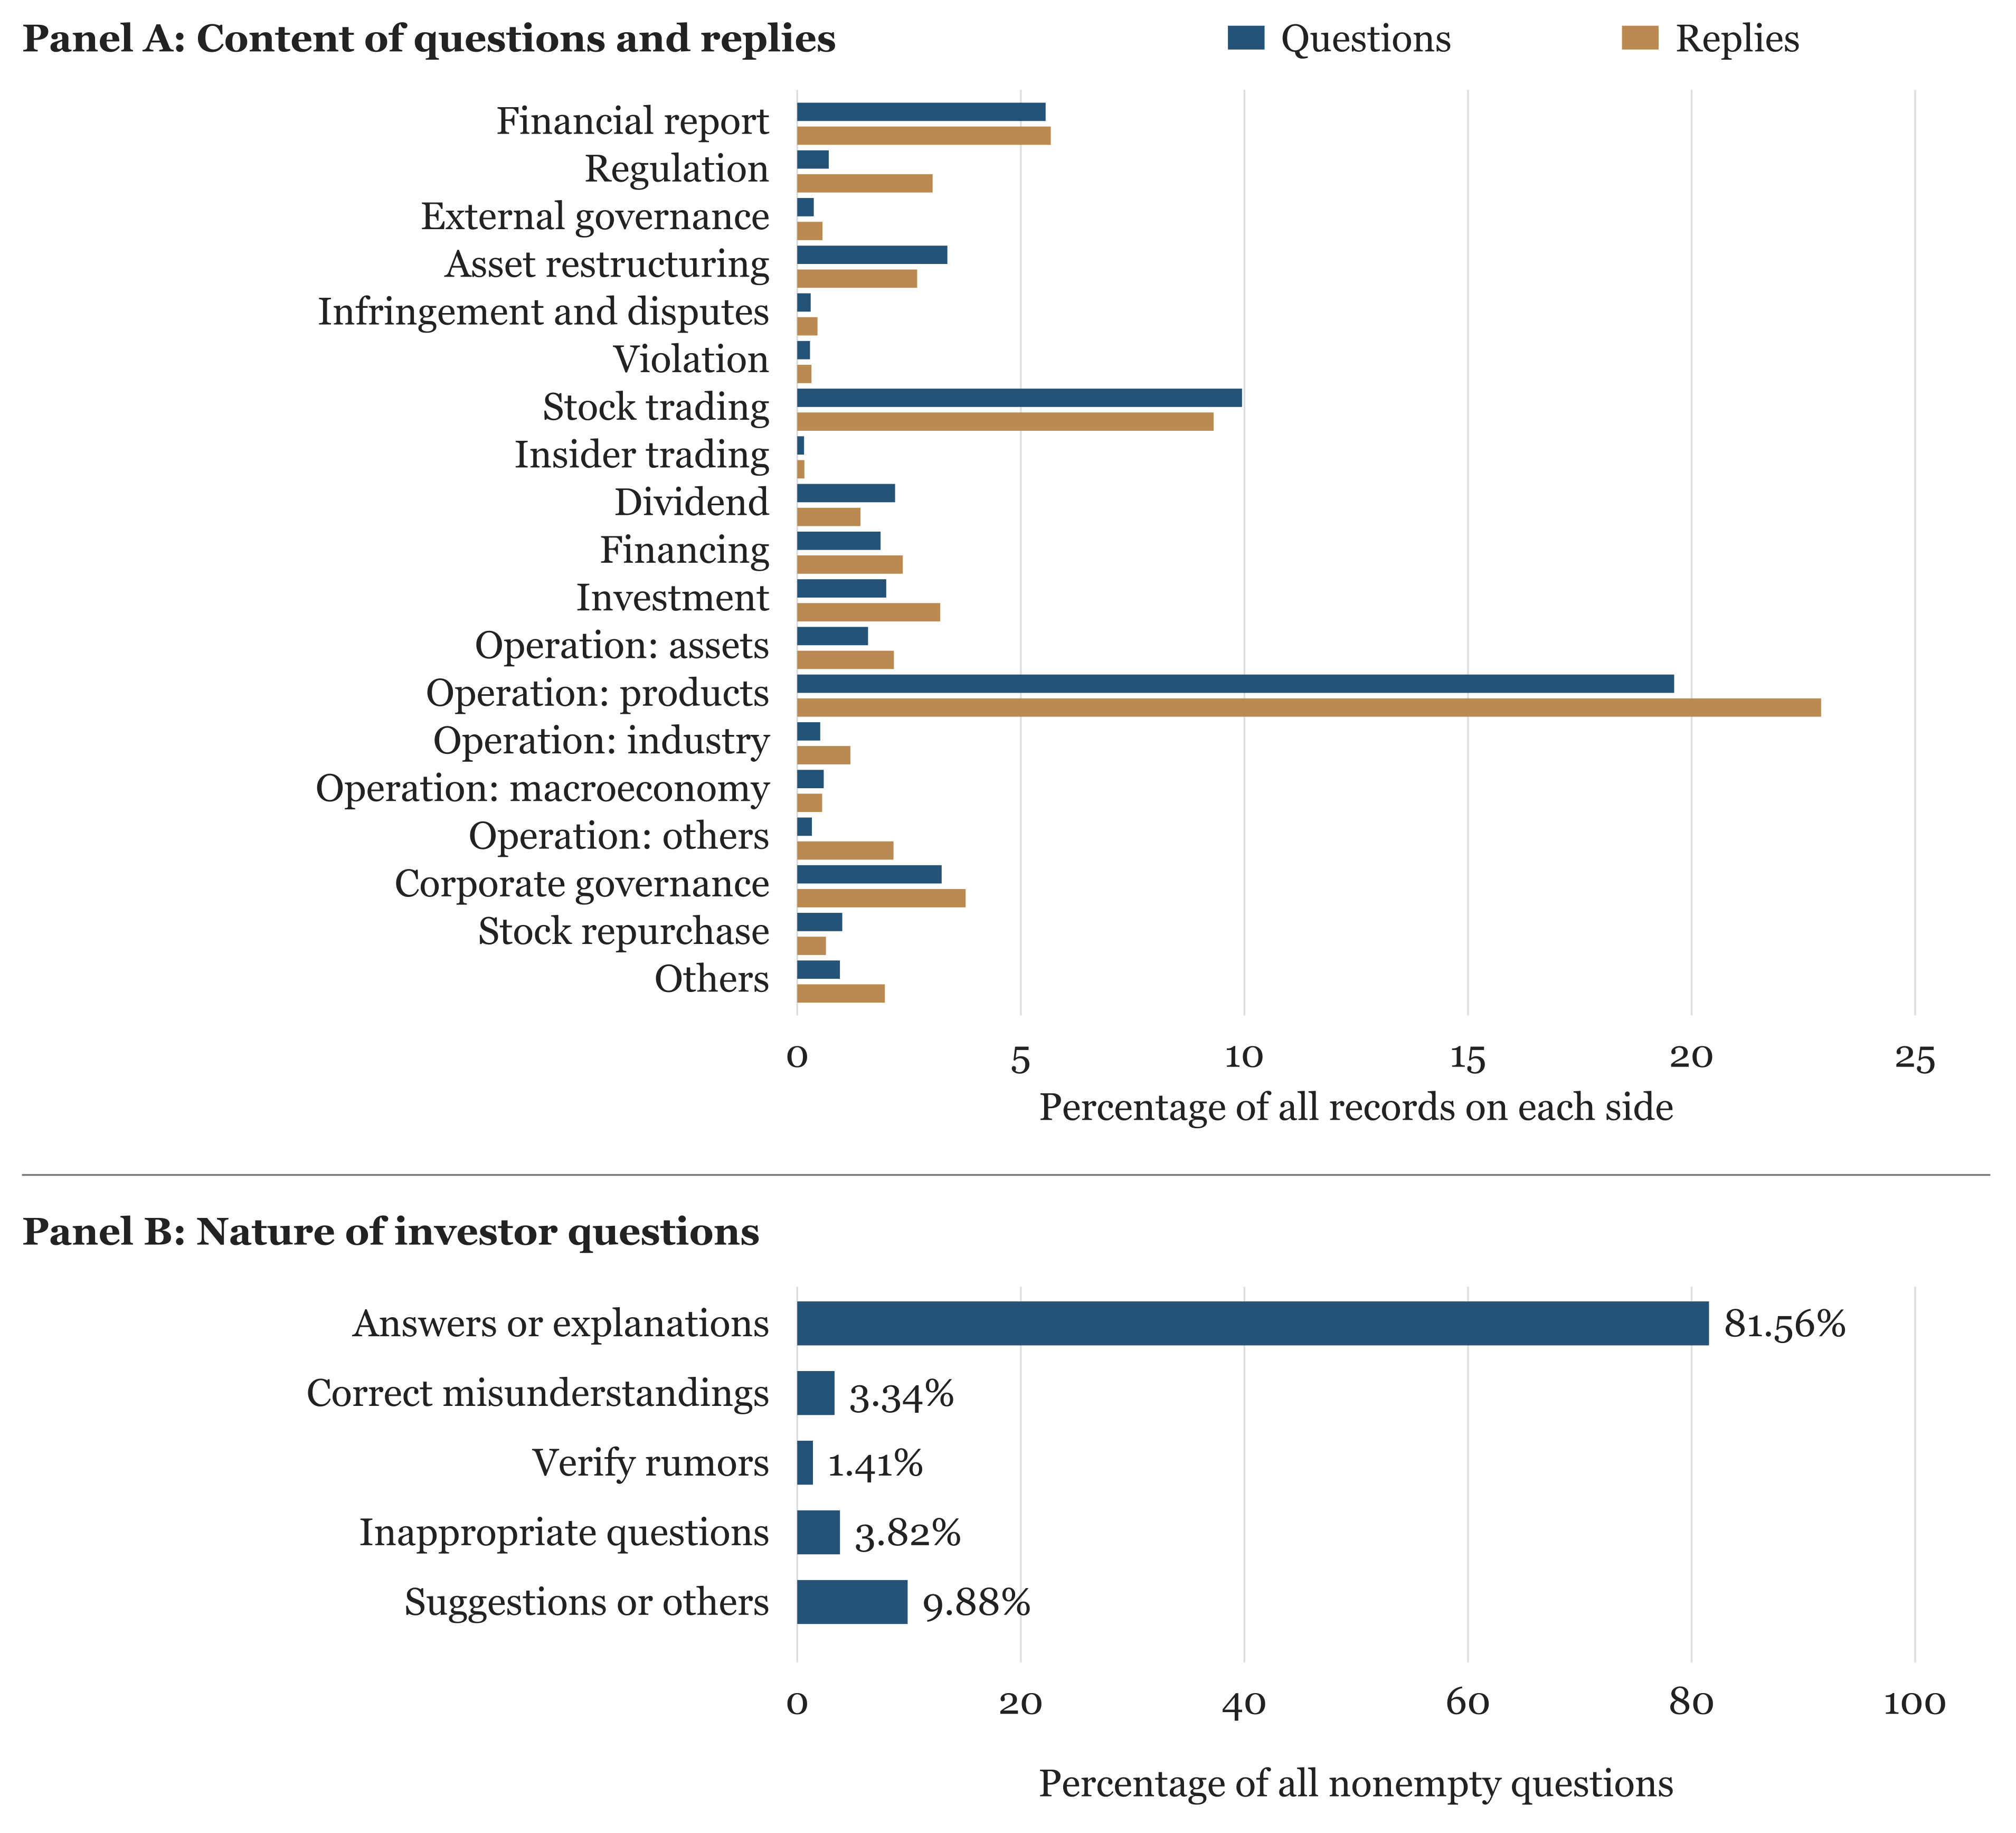
\includegraphics[width=\textwidth]{figures/full_content_and_nature_distribution.png}
\caption{Automated Content and Question Nature Classification}\label{fig:topic_distribution}
\footnotesize Panel A retains the completed question and reply classifications across 19 themes. Its denominator is all source records on each side, including records without an assigned theme, so displayed shares need not sum to 100\%. Panel B uses 5,836,155 nonempty questions. Independent semantic validation remains pending.
\end{figure}

We estimate exploratory C2C slope differences using the dominant question topic at each company-availability date. Let $D_{ik,a}$ indicate category $k$, with unclassified or low-score questions as category 0:
\begin{align}
r^{C2C,e}_{i,a+1}={}&\alpha_i+\delta_a+\beta_0 Z^{ESI}_{i,a}
+\sum_{k=1}^{19}\eta_kD_{ik,a}+\sum_{k=1}^{19}\beta_kZ^{ESI}_{i,a}D_{ik,a}\nonumber\\
&+\boldsymbol c_{i,a}'\boldsymbol\psi+\boldsymbol T_{i,a}'\boldsymbol\rho+\varepsilon_{i,a+1}.\label{eq:topic}
\end{align}
Here $\boldsymbol T$ is omitted in the baseline and contains both tones in the second model. The outcome is next-day C2C excess return, not a CH4 residual. Both models have firm/date effects and two-way clustered errors. Total slopes are $\beta_0$ for category 0 and $\beta_0+\beta_k$ otherwise, in basis points per historical ESI standard deviation.

Table~\ref{tab:full_topic_heterogeneity} retains all 20 categories and both models. Products or business has a baseline slope of 2.02 basis points ($t=3.40$, raw $p=0.000674$, baseline-family BH $p=0.006744$), but 1.12 ($t=1.25$) with both tones. The displayed BH column adjusts the second model's 20 slope tests; its value for this topic is 0.829. Joint slope-equality tests instead test $H_0:\beta_1=\cdots=\beta_{19}=0$, with $p=0.865$ and $0.873$. A significant within-topic slope does not establish a difference from other topics. The analysis remains exploratory.
\begin{table}[H]
\centering
\caption{Exploratory Return Slopes Across Interaction Topics}
\label{tab:full_topic_heterogeneity}
\footnotesize
\renewcommand{\arraystretch}{1.03}
\setlength{\tabcolsep}{3pt}
\begin{threeparttable}
\begin{tabular*}{\textwidth}{@{\extracolsep{\fill}}l c c c c @{}}
\toprule
Dominant Question Content & ESI and Controls & Also Both Tones & BH $p$ & Firm Days \\
\midrule
Unclassified or Low Score & 1.84 (3.44) & 0.97 (1.08) & 0.829 & 180,057 \\
Financial report & 1.04 (0.56) & 0.13 (0.06) & 0.950 & 18,339 \\
Regulation & 5.03 (0.89) & 4.10 (0.72) & 0.829 & 1,125 \\
External governance & -0.15 (-0.01) & -1.16 (-0.07) & 0.950 & 634 \\
Asset restructuring & 3.32 (0.83) & 2.42 (0.60) & 0.829 & 5,507 \\
Infringement, disputes, lawsuit & -8.28 (-0.70) & -9.32 (-0.79) & 0.829 & 738 \\
Violation & -9.77 (-0.62) & -10.83 (-0.69) & 0.829 & 548 \\
Stock trading & 1.22 (1.50) & 0.40 (0.38) & 0.878 & 52,503 \\
Insider trading & -80.80 (-1.10) & -82.10 (-1.11) & 0.829 & 154 \\
Dividend & 1.48 (0.29) & 0.69 (0.13) & 0.950 & 4,169 \\
Financing & -2.47 (-0.59) & -3.44 (-0.80) & 0.829 & 4,590 \\
Investment & 1.84 (0.89) & 0.94 (0.44) & 0.878 & 5,548 \\
Operation operating assets & 2.55 (1.00) & 1.69 (0.64) & 0.829 & 4,681 \\
Operation products or business & 2.02 (3.40) & 1.12 (1.25) & 0.829 & 86,395 \\
Operation industry related & -1.76 (-0.43) & -2.54 (-0.61) & 0.829 & 907 \\
Operation macroeconomic environment & -5.74 (-1.54) & -6.59 (-1.75) & 0.829 & 1,855 \\
Operation others & 3.58 (0.71) & 2.82 (0.55) & 0.829 & 588 \\
Corporate governance & 1.88 (0.45) & 1.05 (0.25) & 0.948 & 5,117 \\
Stock repurchase & 4.07 (0.76) & 3.24 (0.60) & 0.829 & 3,214 \\
Others & -13.17 (-1.36) & -13.81 (-1.42) & 0.829 & 1,057 \\
\midrule
Joint Slope Equality $p$ & 0.865 & 0.873 & -- & -- \\
Adjusted $R^2$ & 0.293 & 0.293 & -- & -- \\
Total Observations & 377,726 & 377,726 & -- & -- \\
\bottomrule
\end{tabular*}\par
\begin{tablenoteblock}
Questions are assigned to 19 fixed content themes and an explicit unclassified category. The dominant category at a firm and availability date is the largest count, including unclassified records. Coefficients are total ESI slopes in basis points per historical standard deviation, not differences from the unclassified reference. Models include category indicators, ESI interactions, baseline controls, and firm and date effects. Errors are clustered by firm and date. The last regression also includes both textual tones. BH probabilities adjust across all topic slopes in that regression. The joint Wald test compares topic slopes rather than counting individually significant estimates. Labels come from assistant supervision and the analysis is exploratory.
\end{tablenoteblock}
\end{threeparttable}
\end{table}


\section{Conclusion}\label{sec:conclusion}
Investor inquiries and managerial replies reveal two sides of public corporate communication. ESI combines their textual direction with attention, reply substantiveness and the investor sentiment state. The reproduced Annual Review specification shows positive one-day O2C associations and larger gross portfolio-return point estimates than either tone alone. Both equal- and value-weighted ESI returns are positive and statistically significant in this historical specification.

The evidence is conditional on the construction and information clock. Assigning later replies to question dates makes the baseline retrospective. When replies must already be public, the complete text horse race and the value-weighted ESI alpha do not establish an incremental advantage. Actual announcement-date tests also do not establish the proposed earnings mechanism. Topic classification describes the content of dialogues, but its joint return tests do not show systematic slope differences and its labels still require independent human validation. These findings motivate further work on information availability and measurement; they do not identify a causal effect of replies, a new priced risk factor, or a reliably implementable strategy.
\clearpage
\bibliographystyle{apalike}
\bibliography{references}
\clearpage
\appendix
\renewcommand{\thetable}{A\arabic{table}}
\setcounter{table}{0}
\renewcommand{\theHtable}{A\arabic{table}}
\section{Public-availability return evidence}
These tables preserve the existing C2C extension and its separate calibration described in Section~\ref{sec:supplements}. They do not use the full-pool historical O2C calibration and do not isolate a single change to the information clock.
\begin{table}[H]
\centering
\caption{Return Predictability after Public Reply Availability}
\label{tab:public_c2c_regressions}
\renewcommand{\arraystretch}{1.02}
\setlength{\tabcolsep}{3pt}
\footnotesize
\begin{threeparttable}
\begin{tabular*}{\textwidth}{@{\extracolsep{\fill}}lcccccc@{}}
\toprule
\multicolumn{7}{@{}l}{\textbf{Panel A: Horse Race Tests for Next Day C2C Excess Returns}} \\
\midrule
Predictor & (1) & (2) & (3) & (4) & (5) & (6) \\
\midrule
ESI & 1.48*** &  &  &  &  & 0.58 \\
 & (4.36) &  &  &  &  & (0.75) \\
Investor Tone &  & -0.15 &  & -0.33 & -0.04 & -0.25 \\
 &  & (-0.22) &  & (-0.48) & (-0.05) & (-0.32) \\
Manager Tone &  &  & 1.84*** & 1.81*** & 1.73*** & 1.10 \\
 &  &  & (4.64) & (4.22) & (3.87) & (1.19) \\
Question Volume &  &  &  & -2.49*** & -2.63*** & -2.59*** \\
 &  &  &  & (-4.18) & (-4.36) & (-4.32) \\
Reply Substantiveness &  &  &  & 0.05 & 0.55 & 0.56 \\
 &  &  &  & (0.09) & (0.76) & (0.78) \\
Question Length &  &  &  &  & 1.23** & 1.24** \\
 &  &  &  &  & (2.43) & (2.45) \\
Reply Length &  &  &  &  & -0.12 & -0.09 \\
 &  &  &  &  & (-0.17) & (-0.12) \\
Q\&A Similarity &  &  &  &  & -0.65 & -0.66 \\
 &  &  &  &  & (-1.13) & (-1.15) \\
\midrule
Controls, Firm FE, Date FE & Yes & Yes & Yes & Yes & Yes & Yes \\
Observations & 377,721 & 377,721 & 377,721 & 377,721 & 377,721 & 377,721 \\
Adjusted $R^2$ & 0.293 & 0.293 & 0.293 & 0.293 & 0.293 & 0.293 \\
\bottomrule
\end{tabular*}\par
\begin{tablenoteblock}
All columns use the same 377,721 observations from 2017 through 2024. The outcome runs from close $a$ to close $a+1$, where $a$ is the first trading day strictly after the last recorded reply. Coefficients are in basis points. Investor and managerial tone and ESI use their historical calibration scales. Other text features and controls are centered and scaled within the availability panel without using return outcomes. All columns include the baseline controls in Section \ref{sec:baseline_return_predictability}, firm effects, and date effects. Standard errors are clustered by firm and date. Adjusted $R^2$ accounts for the regressors and absorbed effects. The unrounded adjusted $R^2$ change from column (5) to column (6) is $-0.000000888$. ***, **, and * denote nominal significance at 1\%, 5\%, and 10\%, respectively.
\end{tablenoteblock}
\end{threeparttable}
\end{table}
\clearpage
\begin{table}[H]
\centering
\ContinuedFloat
\caption{Return Predictability after Public Reply Availability (continued)}
\renewcommand{\arraystretch}{1.02}
\setlength{\tabcolsep}{3pt}
\footnotesize
\begin{threeparttable}
\begin{tabular*}{\textwidth}{@{\extracolsep{\fill}}lcccccc@{}}
\toprule
\multicolumn{7}{@{}l}{\textbf{Panel B: Panel OLS across Horizons}} \\
\midrule
Predictor & 1 Day & 5 Days & 10 Days & 20 Days & 40 Days & 60 Days \\
\midrule
ESI & 1.48*** & 4.04*** & 6.63*** & 5.08*** & 8.11*** & 10.29*** \\
 & (4.36) & (4.80) & (5.57) & (2.82) & (2.94) & (2.94) \\
Investor Tone & -0.16 & -1.30 & -2.61 & -9.76*** & -5.69 & -4.74 \\
 & (-0.23) & (-0.79) & (-1.13) & (-2.91) & (-1.14) & (-0.74) \\
Manager Tone & 1.84*** & 5.56*** & 9.37*** & 9.47*** & 14.69*** & 18.22*** \\
 & (4.64) & (5.59) & (6.55) & (4.44) & (4.46) & (4.01) \\
Question Volume & -2.53*** & -9.00*** & -15.52*** & -14.14*** & -12.74** & -15.42* \\
 & (-4.23) & (-6.11) & (-6.94) & (-4.37) & (-2.26) & (-1.77) \\
Reply Substantiveness & 1.25** & 3.18*** & 7.81*** & 10.08*** & 11.67*** & 14.91*** \\
 & (2.54) & (2.61) & (4.30) & (3.62) & (2.87) & (2.70) \\
\midrule
Controls & Yes & Yes & Yes & Yes & Yes & Yes \\
Firm FE and Date FE & Yes & Yes & Yes & Yes & Yes & Yes \\
Observations & 377,726 & 375,668 & 373,415 & 368,682 & 358,630 & 349,301 \\
Adjusted $R^2$ & 0.293 & 0.325 & 0.333 & 0.333 & 0.342 & 0.341 \\
\midrule
\multicolumn{7}{@{}l}{\textbf{Panel C: Fama and MacBeth Regressions}} \\
\midrule
Predictor & 1 Day & 5 Days & 10 Days & 20 Days & 40 Days & 60 Days \\
\midrule
ESI & 1.00*** & 3.63*** & 6.01*** & 7.35*** & 13.44*** & 18.90*** \\
 & (2.86) & (4.14) & (4.36) & (3.64) & (4.24) & (4.07) \\
Investor Tone & -0.04 & 0.34 & 0.32 & -1.04 & 10.64** & 23.45*** \\
 & (-0.07) & (0.22) & (0.14) & (-0.31) & (2.15) & (3.31) \\
Manager Tone & 1.26*** & 4.57*** & 8.29*** & 11.20*** & 19.64*** & 25.80*** \\
 & (3.05) & (4.43) & (5.25) & (4.74) & (4.98) & (4.36) \\
\midrule
Controls & Yes & Yes & Yes & Yes & Yes & Yes \\
Observations & 377,444 & 375,392 & 373,148 & 368,429 & 358,397 & 349,074 \\
Daily Cross Sections & 1,452 & 1,448 & 1,443 & 1,433 & 1,413 & 1,393 \\
Adjusted $R^2$ & 0.103 & 0.124 & 0.127 & 0.114 & 0.098 & 0.095 \\
\bottomrule
\end{tabular*}\par
\begin{tablenoteblock}
The outcome is the cumulative total stock return minus the cumulative risk free return from close $a$ to close $a+h$, with complete observations for every holding day. Each signal enters a separate regression with the baseline controls. The observations and adjusted $R^2$ in each column refer to the ESI specification. Panel B uses firm and date effects and standard errors clustered by firm and date. Panel C averages estimable daily cross-sectional slopes. Its HAC standard errors use $\max(5,h)$ exchange trading day lags, retaining missing estimation dates as calendar gaps. The reported adjusted $R^2$ is the mean across these daily regressions. Coefficients are in basis points and $t$ statistics appear in parentheses. Stars denote nominal significance and do not adjust for the correlated horizon tests.
\end{tablenoteblock}
\end{threeparttable}
\end{table}

\clearpage
\begin{table}[H]
\centering
\caption{Portfolio Returns after Public Reply Availability}
\label{tab:public_c2c_portfolios}
\renewcommand{\arraystretch}{1.02}
\setlength{\tabcolsep}{3pt}
\footnotesize
\begin{threeparttable}
\begin{tabular*}{\textwidth}{@{\extracolsep{\fill}}lcccccc@{}}
\toprule
\multicolumn{7}{@{}l}{\textbf{Panel A: Equal Weights}} \\
\midrule
Signal & Long (bps) & Short (bps) & Ann. Ret (\%) & Sharpe & CH4 $\alpha$ & FF3 $\alpha$ \\
\midrule
ESI & 5.38 & 1.24 & 10.56 & 1.11 & 4.68*** (3.29) & 4.33*** (3.09) \\
Investor Tone & 1.70 & 2.59 & -2.13 & -0.22 & 0.09 (0.07) & -0.85 (-0.59) \\
Manager Tone & 5.17 & 0.69 & 11.46 & 1.15 & 4.75*** (3.18) & 4.65*** (3.13) \\
\midrule
\multicolumn{7}{@{}l}{\textbf{Panel B: Value Weights}} \\
\midrule
Signal & Long (bps) & Short (bps) & Ann. Ret (\%) & Sharpe & CH4 $\alpha$ & FF3 $\alpha$ \\
\midrule
ESI & 2.71 & -0.13 & 7.13 & 0.43 & 3.78 (1.54) & 3.09 (1.27) \\
Investor Tone & 0.15 & 0.85 & -1.67 & -0.10 & 0.79 (0.32) & -0.38 (-0.15) \\
Manager Tone & 4.24 & -2.04 & 16.42 & 0.90 & 6.85*** (2.71) & 6.50** (2.57) \\
\bottomrule
\end{tabular*}\par
\begin{tablenoteblock}
All three signals use the same daily candidate stock pool and the same 1,786 complete return dates from 2017 through 2024. The information date $a$ is the first trading day strictly after the last recorded reply. Each long leg selects up to 50 stocks with positive signals from the upper 30 percent of the distribution. Each short leg selects up to 50 stocks with negative signals from the lower 30 percent. Returns run from close $a$ to close $a+1$ and include cash dividends. Long and Short are gross excess returns in basis points. Annualized return is $100[\exp(242\overline{r}^{LS})-1]$, and Sharpe uses 242 trading days. Value weights use lagged market capitalization. CH4 and the domestic FF3 factors cover the same holding day. FF3 uses CSMAR market P9714 and the circulating market capitalization series RiskPremium1, SMB1, and HML1. Alphas are in basis points, with HAC $t$ statistics using five exchange trading day lags in parentheses. Missing return dates are retained as gaps in the HAC calendar. The short leg is theoretical, and returns exclude trading and borrowing costs. ***, **, and * denote nominal significance at 1\%, 5\%, and 10\%, respectively.
\end{tablenoteblock}
\end{threeparttable}
\end{table}


\section{Text model assessment}\label{app:nlp_methodology}
The common-holdout exercise compares reply substantiveness predictions against the same labels. Normalized reply templates remain in one partition; model ranking uses no stock-return criterion. Chinese BERT achieves the highest macro F1, but agreement with existing labels is not independent semantic accuracy. The benchmark BERT is not the undocumented production model underlying all sentiment scores. Replacing production substantiveness would change ESI and requires a separately specified study; no partial replacement is made here.
\begin{table}[H]
\centering\footnotesize
\caption{Reply Substantiveness: Common-Holdout Model Comparison}\label{tab:substantiveness_benchmark}
\begin{threeparttable}
\renewcommand{\arraystretch}{1.12}
\begin{tabular*}{\textwidth}{@{\extracolsep{\fill}}lrrrrr@{}}
\toprule
Model & Macro F1 & Balanced acc. & AUC & Brier & ECE \\
\midrule
Random Forest & 0.707 & 0.706 & 0.800 & 0.174 & 0.057 \\
Chinese BERT benchmark & 0.827 & 0.830 & 0.913 & 0.117 & 0.071 \\
Local instruction LLM & 0.440 & 0.455 & 0.433 & 0.283 & 0.204 \\
\bottomrule
\end{tabular*}
\begin{tablenoteblock}
The same 402 existing-label test pairs are used for every model. The 1,999 usable labels are split into 1,280 training, 317 validation and 402 test pairs with no normalized reply template shared across partitions. Higher F1, balanced accuracy and AUC, and lower Brier and ECE, indicate better agreement with these labels. Annotator identifiers, a complete labeling protocol, and inter-rater agreement are unavailable; this is not independent semantic ground truth. The original Random Forest score is retained in the return tests, with no selective replacement by BERT predictions.
\end{tablenoteblock}
\end{threeparttable}
\end{table}


\section{Variable definitions}\label{app:variable_definitions}
\begin{table}[H]\centering\footnotesize
\caption{Variables Grouped by Empirical Use}\label{tab:variables}
\renewcommand{\arraystretch}{1.15}
\begin{tabularx}{\textwidth}{@{}p{.25\textwidth}X@{}}
\toprule Variable & Definition and use\\\midrule
\multicolumn{2}{l}{\textbf{Text signals}}\\
Investor and manager tone & Mean positive-minus-negative sentiment probability for each side of the matched cohort.\\
Reply substantiveness & One minus the production Random Forest evasiveness probability.\\
Question volume & Number of questions; normalized logarithm scales the historical investor component.\\
ESI & Equation~\eqref{eq:esi}; standardized using original regression-pool moments in the baseline regressions.\\
Lengths and similarity & Question and reply lengths and Q\&A similarity, added in the availability horse race.\\\midrule
\multicolumn{2}{l}{\textbf{Baseline outcomes and controls}}\\
O2C excess return & Next-record close/open minus one, less that record's risk-free return.\\
CH4 or q5 residual & Original full-period firm OLS residual using signal-date factors.\\
Size, BM, ROA, Lev & Log capitalization, book-to-market, profitability and leverage in the inherited master panel.\\
Illiquidity, turnover & Inherited Amihud measure and turnover variable, retaining original units.\\
Return controls & Lag-one return; sum from records $t-30$ to $t-2$ (29 records, at least 10); preceding 30-record volatility (at least 10).\\
News tone and indicator & Prior media tone and coverage over the inherited $t-30$ to $t-3$ window.\\\midrule
\multicolumn{2}{l}{\textbf{Supplement-specific quantities}}\\
Maximum reply lag & Largest reply-date minus question-date natural-day interval within the original cohort.\\
Availability date & First exchange trading day strictly after the last recorded reply.\\
C2C excess return & Total close-to-close stock return less risk-free return over the same holding interval.\\
SUE, Annodt & Original CSMAR standardized unexpected earnings and actual report publication date, not an update-date proxy.\\
Dominant topic & Largest question-category count at the company-availability date, including unclassified records.\\
\bottomrule\end{tabularx}
\end{table}

\section{Replication scope and unresolved evidence}
This draft replaces printed baseline figures with verified recomputations. The principal positive finding is the one-day historical association. The repository includes aggregate outputs, code, table generators, notebook entry points and a claim-to-source map. Licensed raw and company-level data, original teacher annotations, model weights and record-level text remain local. Replication from frozen prepared data is distinguished from rebuilding licensed raw ingestion.

The original multi-horizon O2C tables, conditional sorts, parameter-grid results, message-board analyses and trade-size mechanisms remain archived pending reconciliation. This is an evidence-status decision, not selection based on significance. Their exclusion from the active evidence set is not a new rejection or confirmation of the associated hypotheses. Parameters, variables and samples were not changed to recover old significance.

Archived trade-size variables distinguish large and small trades, not verified institutional and retail accounts. Future re-estimation should define their difference before coefficient comparisons and distinguish one-day from five-day windows. Claims that order flow identifies institutional information processing, insider-sale results rule out opportunism, or crash outcomes establish credibility are not carried forward without verified support. A matched-specification historical O2C full-text horse race and complete multi-horizon reconciliation remain research tasks. Independent semantic validation, accounting vintages and implementability analysis are also needed before stronger conclusions can be drawn.

\end{document}
